\documentclass{beamer}

\usepackage{tikz}
\usepackage{amsthm}
\usetheme{metropolis}

\title{TODO: my awesome title}
\subtitle{TODO: snarky comment here}
\author{Murray Heymann\\15988694}
\institute{University of Stellenbosch}
\date{3 October 2017}

%\definecolor{USmaroon}{rgb}{0.55555, 0.058888, 0.17}
%\usecolortheme[named=USmaroon]{structure}


\setbeamertemplate{navigation symbols}{}

\setbeamertemplate{bibliography item}{\insertbiblabel}


\theoremstyle{definition}
\newtheorem*{thrm}{Theorem}


\begin{document}


\begin{frame}
	\titlepage
\end{frame}

\section{Definitions}

\begin{frame}
	\frametitle{Partitions}
	\begin{definition}
		Let $S$ be a set.
		A partition $P$ of $S$ is a set of subsets of $S$ such that 
		\begin{align}
			S &= \cup\{x : x \in P\}\\
			x \in P &\Rightarrow x \not = \emptyset\\
			x, y \in P &\Rightarrow\ x = y \vee x \cap y = \emptyset.
		\end{align}
	\end{definition}
\end{frame}

\begin{frame}
	\frametitle{Equivalence Relations}
	\begin{definition}
		Let $S$ be a set.  An equivalence relation $R$ is a set of ordered
		pairs of elements of $S$ with the following properties
		\begin{align}
			a \in S &\Rightarrow (a, a) \in R\\
			(a, b) \in R &\Rightarrow (b, a) \in R\\
			\label{trans}(a, b) \in R, (b, c) \in R &\Rightarrow (a, c) \in R.
		\end{align}
		Note the notational variation $(a, b) \in R \Leftrightarrow aRb$.
	\end{definition}
\end{frame}

\begin{frame}
	\frametitle{Equivalence class}
	\begin{definition}
		Let $S$ be a set and $R$ be an equivalence relation of elements of
		$S$. Further, let $a$ be an element of $S$. An equivalence class of
		$a$, denoted by $[a]$, is the set of all elements that are equivalent
		to $a$ under $R$
		\begin{align}
			[a] := \{x \in S : (a, x) \in R\}
		\end{align}

	\end{definition}
\end{frame}
	

\begin{frame}
	\frametitle{Bijection}
	\begin{definition}
		A Bijection is a mapping $f$ between elements two sets $X$ and
		$Y$, where
		\begin{align}
			\label{fx:domain}\forall x \in X&,\ \exists y \in Y\ \text{s.t.}\
			f(x) = y\\
			\label{fx:uniq}f(x) = y_{1}&,\ f(x) = y_{2} \Rightarrow y_{1} =
			y_{2}\\
			\forall y \in Y&,\ \exists x \in X\ \text{s.t.}\ f(x) = y\\
			f(x_{1}) = y&,\  f(x_{2}) = y \Rightarrow x_{1} = x_{2}
		\end{align}
		Note that (\ref{fx:domain}) and (\ref{fx:uniq}) implies f is
		actually a function with domain $X$ and codomain $Y$.
	\end{definition}
\end{frame}


\section{Theorems}

\begin{frame}
	\frametitle{Fundamental theorem of equivalence relations}

	\begin{thrm}
		Any Equivalence $R$ relation on a set $S$ partitions $S$. Conversely, for
		any partition on $S$, there exists a corresponding equivalence
		relation $R$ on $S$.
	\end{thrm}

\end{frame}

\begin{frame}
	\frametitle{Fundamental theorem of equivalence relations}
	\begin{proof}
		We show that there exists a bijection between the set of all
		partitions $\mathbf{P}$ of $S$ and the set of all equivalence
		relations $\mathbf{R}$ of $S$.
		\begin{itemize}
			\item
				Let $P \in \mathbf{P}$. This maps to the equivalence 
				relation $R \in \mathbf{R}$ where $aRb \Leftrightarrow \exists p \in
				P\ \text{s.t.}\ a,b \in p $
			\item
				Let $R \in \mathbf{R}$. 
				\begin{itemize}
					\item
						Consider the set $\{[x]: x \in S\}$. 
					\item
						Let $x, y\in S$ and assume $[x] \cap [y] \not =
						\emptyset$.  
					\item
						If $c \in [x] \cap [y]$ and $x^{\prime} \in [x]$
						then $x^{\prime}Rc$ and $cRy$
						and by (\ref{trans}) $x^{\prime}Ry$.  It follows that $[x]
						\subseteq [y]$.  
					\item
						By symetry, $[y] \subseteq [x]$ and
						therefore $[x] = [y]$. Note that none of the equivalence
						classes can be the empty set. Clearly $\cup_{x \in S} [x] =
						S$. 
					\item
						We conclude that $\{[x]: x \in S\}$ is a partition of
				$S$ under $R$
				\end{itemize}
		\end{itemize}
	\end{proof}
\end{frame}

\begin{frame}
	\frametitle{Another one}


	\begin{itemize}
		\item
			One Ring to rule them all
		\item
				One Ring to find them
		\item
			One Ring to bring them all
		\item
			And in the darkness bind them
	\end{itemize}
\end{frame}

\begin{frame}
	\frametitle{T\textit{i}kZ}
\end{frame}
\begin{frame}
	\frametitle{T\textit{i}kZ}
	\url{texample.net}

	\begin{figure}
		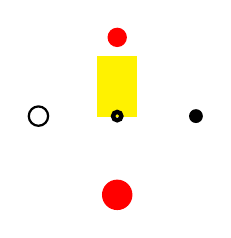
\begin{tikzpicture}[scale=0.5]
		\fill[yellow,draw] (-0.5,0) rectangle (0.5,1.5);
			\draw[ultra thick] (0,0) circle (3pt);
			\draw[thick] (-2, 0) circle(7pt);
		\fill (2,0) circle (5pt);
		\fill[red] (0, 2) circle (7pt)
				   (0,-2) circle (11pt);
	\end{tikzpicture}
		\caption{A T\textit{i}kZ drawing}
	\end{figure}
\end{frame}

\begin{frame}
	\frametitle{Connecting things}

	\begin{figure}
		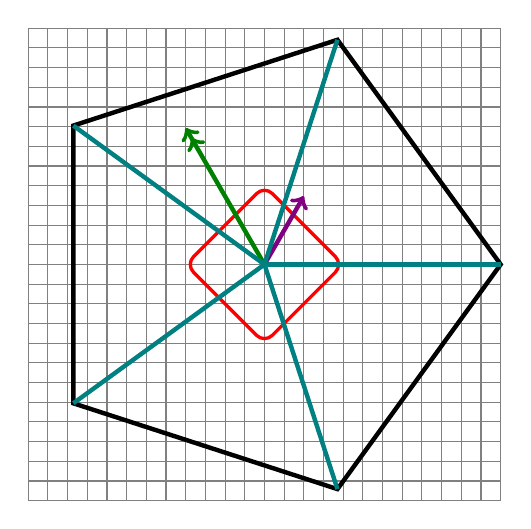
\begin{tikzpicture}
			\draw[step=0.25, color=gray] (-3,-3) grid (3,3);
			\draw[very thick, red, rounded corners]
				(1,0) -- (0, 1) -- (-1, 0) -- (0, -1) -- cycle;
			% color mixing below:  50 % blue, complement red
			\draw[ultra thick, blue!50!red, ->] 
				(0,0) -- (60:1cm);
			\draw[ultra thick, green!50!black, ->>] (0,0) -- (120:2cm);
			\path (0:3cm) coordinate (P0);
			\path (1*72:3cm) coordinate (P1);
			\path (2*72:3cm) coordinate (P2);
			\path (3*72:3cm) coordinate (P3);
			\path (4*72:3cm) coordinate (P4);
			\draw[ultra thick] (P0) -- (P1) -- (P2) -- (P3) -- (P4) -- cycle;
			\foreach \i in {0,...,4}
				\draw[ultra thick, blue!50!green] (0,0) -- (P\i);
		\end{tikzpicture}
		\caption{bla\cite{boom}}
	\end{figure}
\end{frame}

\begin{frame}
	\frametitle{References}
	\begin{thebibliography}{1}
		\bibitem{koblitz} Kobliz
		\bibitem{boom} Boom
	\end{thebibliography}
\end{frame}

\end{document}
